\documentclass[conference]{IEEEtran}
\IEEEoverridecommandlockouts
% The preceding line is only needed to identify funding in the first footnote. If that is unneeded, please comment it out.
\usepackage{cite}
\usepackage{amsmath,amssymb,amsfonts}
\usepackage{algorithmic}
\usepackage{graphicx}
\usepackage{textcomp}
\usepackage{hyperref}
\usepackage{xcolor}
\usepackage{array}
\def\BibTeX{{\rm B\kern-.05em{\sc i\kern-.025em b}\kern-.08em
    T\kern-.1667em\lower.7ex\hbox{E}\kern-.125emX}}
\begin{document}

\title{Deep Neural Network Image Classifier for an NVIDIA Graphical Processing Unit}

\author{\IEEEauthorblockN{Brian Curless\IEEEauthorrefmark{1}, Brandon Mack\IEEEauthorrefmark{2}, Eli Barela\IEEEauthorrefmark{3}, and Evan Palmisano\IEEEauthorrefmark{4}} 
\IEEEauthorblockA{School of Informatics, Computing, and Cyber Systems \\
Northern Arizona University, Flagstaff, Arizona, USA \\
Email: \IEEEauthorrefmark{1}bc2497@nau.edu, \IEEEauthorrefmark{2}bjm462@nau.edu, \IEEEauthorrefmark{3}ejp243@nau.edu, \IEEEauthorrefmark{4}emb538@nau.edu}}
%bjm462@nau.edu}
%emb538@nau.edu}
%ejp243@nau.edu}


\maketitle

\begin{abstract}
Training deep neural networks is a computationally intensive workload. A typical multi-layer neural network used for image classification is made up of many large matrix multiplications, two dimensional convolutions, and other massively parallel computations. A vast amount of training data must also be transferred through the network for parameter optimization. Transferring this quantity of data requires a high memory bandwidth. We created a programming framework designed to run on an NVIDIA graphical processing unit that is able to efficiently and quickly train a deep neural network for image classification. The framework supports fully connected layers, rectified linear unit nonlinearities, and a softmax classifier. It is also designed to be easily extensible where layers can be added, removed, or reordered. For example a series of convolutional and max pool layers could be created following our programming paradigm. We prove the framework's effectiveness by training two separate network architectures for image classification on the CIFAR-10 dataset and report the results here.
\end{abstract}

\begin{IEEEkeywords}
neural network, graphics, GPU, image classifier
\end{IEEEkeywords}

\section{Introduction}

Our team is studying how to create an image classifier using the graphics processing unit (GPU) as much as possible and comparing it to contemporary programs that are implemented using the GPU. Not only do we wish to see if our implementation is faster than these contemporaries, but we also wish to observe if our program will be effective in determining the classification of an image. To do so, we will be training, validating, and testing our program using the CIFAR-10 image set of 32 x 32 pixel images. Any contemporary programs must also adhere to using CIFAR-10 exclusively in testing the model. As for our program solely, it is a program that takes a layered approach to creating a neural network which trains to properly identify which of the 10 classes of the CIFAR-10 dataset an image belongs to.

\section{Background}

We started this project by looking in the textbook \textit{Programming Massively Parallel Processors: Fourth Edition} by Wen-mei W. Hwu, David B. Kirk and Izzat El Hajj\cite{b1}. Chapter 16 of this book focuses on deep learning algorithms, or at least a part of the process. Namely, this chapter focuses on utilizing the GPU to create a convolutional layer for deep learning algorithms, as opposed to how to construct such a program from scratch. As such, after coming to the conclusion the text book wouldn't be able to guide us, we had to begin looking elsewhere for valuable information regarding neural networks. We ultimately deferred to Brian Curless, who has experience working on image classifier programs through prior classwork. He decided that for our neural network group, a simple layered approach to an image identifier would be optimal. Brian received much of his information in kind through both past experience and by introducing us to resources from Stanford University\cite{b3}, wherein we were exposed to the concept behind making an image classifier that continues to learn and grow over time. In contrast to the information presented to us, we resolved to use a GPU kernel for computations at each layer, thereby using parallel processing to achieve the same results but in a fashion we hoped would be much faster.

\section{Description of our Approach}

When designing our image classifier, we decided to use a layered architecture that would allow us to build as much or as little as we wished to create the program. This layered architecture ultimately ended up being a dual layer classifier with weights trained through stochastic gradient descent (SGD). This dual layer classifier makes usage of several important pieces to train, validate, and test the data from the CIFAR-10 dataset, which also required a special import process for the information.

\begin{figure}[htbp]
\centerline{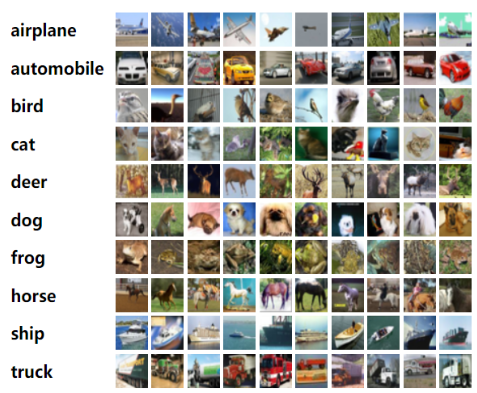
\includegraphics[width=75mm]{cifar_categories.png}}
\caption{CIFAR-10 Example Sheet}
\label{CIFAR}
\end{figure}

The Neural Network functions as follows:

\begin{enumerate}
    \item The CIFAR 10 dataset is loaded into memory.
    \item The parameters and intermediate values for the network are all allocated on the GPU in global memory.
    \item Initial, random values are generated for parameters, and they are copied to the GPU.
    \item A randomly sampled minibatch of images is grabbed from the 'train' dataset and copied to the input of the network.
    \item The forward API is invoked on all layers (which in turn launch their own kernels internally).
    \item The softmax loss is calculated, and the gradient with respect to the loss is calculated.
    \item The upstream gradient is backpropagated through the entire network through the backward API of each layer.
    \item The gradient of the loss with respect to the parameters is then used to update the parameters. A momentum based approach is used to speed up convergence.
    \item The process is repeated for as many epochs are specified in the program.
    \item Once training is complete, hyper parameters are tuned iteratively using cross validation on a set of 10,000 validation images.
    \item Finally, a set of 10,000 test images that were reserved are used to determine the effectiveness of the model.
\end{enumerate}

We implemented two different network topologies following this strategy. The first of which is a single layer linear classifier that will herein be referred to as the "Single Layer Classifier", or just "Single Layer" . The output scores of the network are computed as follow:
\begin{equation}\label{eq:singleLayer}
y_{\text{single}}=W \cdot x + b
\end{equation}

This network is just a simple linear predictor that is trained using stochastic gradient descent. It was created as a stepping stone to prove out the rest of our code before creating a multi layer network. 

The second network topology we implemented was a two layer neural network which will be referred to as the "Dual Layer Classifier", or just "Dual Layer". It's output scores are calculated as follows: 
\begin{equation}\label{eq:dualLayer}
y_{\text{dual}}=W_2 \cdot \text{max}(0, W_1 \cdot x + b_1) + b_2
\end{equation}

This network has two linear layers with weights $W_1$, $W_2$, biases $b1$, $b_2$, and a ReLU activation unit placed in between the layers. The nonlinear activation function is very important because without it the network would reduce to our single layer topology. The ReLU activation function thresholds any negative activations to zero, and preserves the other inputs. The ReLU activation function allows each hidden layer neuron to behave independent of the previous layer neurons. Instead of attempting to create simple hyperplane boundaries for each class as in the single layer network, the dual layer network can use it's hidden layer to transform the input space to a more favorable, and more easily separable space. Each of the components that we used in creating these two networks will be expounded in the subsections following.


\subsection{Data Gathering and Storage}

As stated previously, we are using the CIFAR-10 dataset\cite{b2} in order to train, validate, and test our image classifier. In order to do so, the data must first be divided into various parts, so that each dataset avoids using the same images more than once. The CIFAR-10 dataset is divided across 6 files, each sporting 10,000 images which are each comprised of 32 x 32 = 1024 pixels and a specifier. As such, we decided to use 40,000 images to train or 4 files, with 10,000 images being assigned to validation and 10,000 more being assigned to testing. After dividing the images, the images must be imported in a readable way for the computer, accomplishing the creation of the neural network portion. Within the CIFAR-10 files, the 10,000 images are stored within binary files, with each image taking up 3073 bytes of information. The first byte represents an integer from 0-9 which specifies what the image is supposed to represent. From here, the remaining 3072 bytes are divided into 3 groups of 1024 bytes, with each group representing red, green, and blue values respectively for each of the 1024 pixels in an image. As these are each 1 byte, and the maximum value for each color is 255, each byte is an unsigned integer comprised of 8 bits. Using a C++ program, each byte is read from a file into a temporary character variable. This character is then cast to an unsigned character before either being cast as an unsigned integer for the specifier byte, or cast as a float value (more reason on this later). After the recast of the imported information, the new values are placed into vectors within a custom structure. This structure has 6 members: xTrain, yTrain, xVal, yVal, xTest, and yTest. Each of the x vectors are of type float and hold the RGB (red, green, blue) values for each pixel of every image in each of the datasets for training, validation, and testing. The y vectors are of type unsigned integer 8 bit in C and holds each value that is meant to correspond to each set of RGB values as the specifier byte.

\begin{figure}[htbp]
\centerline{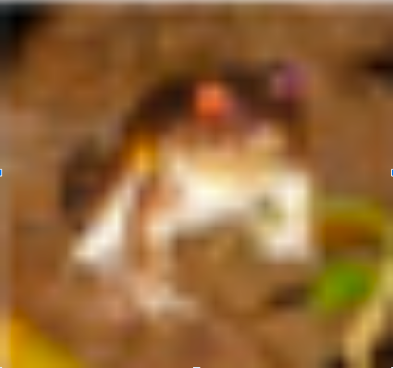
\includegraphics[width=75mm]{frog_cifar.png}}
\caption{CIFAR-10 Image 1, File 1, Type Frog}
\label{frog}
\end{figure}

\subsection{Affine Layer}
The Affine Layer, otherwise known as a fully connected layer, is an important component of neural networks. It's purpose is to be the bridge between the input data and the subsequent layers. It is responsible for transforming the input through a linear operation. In the affine layer, each neuron is connected to every neuron in the preceding layer which forms a dense network of connections. By applying a matrix multiplication between the input data and a table of weights with an addition of a bias, the neural network can learn complex patterns and relationships within the data, making the affine layer necessary for the effectiveness of the neural network in tasks which includes our project of classification.

\subsubsection{Forward Pass}
Applying matrix multiplication to our project is crucial. The affine forward function performs this for us by multiplying our dataset by our weights table and adding a bias value for every cell of the output table. The function performs non-symmetrical matrix multiplication due to the batch size and output matrix sizes being dynamic. It is dependent with the batch size which is how many images are being processed at once.

Each of these matrix multiplications computes $y$ where $$y=Wx+b$$ and $y$ is a matrix of size $(\text{numOutputs} 
 \times \text{batchSize})$ and $x$ is a matrix of size $(\text{inputDataSize} 
 \times \text{batchSize})$. A vector $b$ that is $(\text{numOutputs}\times 1)$ is used to provide a bias term for each output. Based on the sizes of $x$ and $y$, $W$ must be $(\text{numOutputs} 
 \times \text{dataSize})$. 

 To compute $y_{i,j}$ we allocate $N$ threads where $N = i * j$. Each thread will compute the inner product of one vector of input data $x$, namely the $j_\text{th}$ column of $x$, and the $i_\text{th}$ row of $W$. $$y_{i,j}=\sum_{k=0}^{dataSize-1}{x_{k,j}*W_{i,k}}$$ 
 
 This equation is applied to a single for loop that iterates over dataSize and multiplies the appropriate value of $x$ and $W$, and accumulates the result into a register for that thread. After the multiplication occurs, $b$ is added to the multiplication result, and the value is assigned to the output vector $f$. An optimization to consider is to allocate and launch a 2D grid of threads that is greater than the size of the output matrix. Due to the dynamic data sizes, the kernel might experience thread starvation.

\subsubsection{Backward Pass}
All layers in our network need to be able to compute the gradient of the loss with respect to the inputs to the layer. As stated above, the affine layer has a weight matrix $W$, a bias vector $b$, a batch of input vectors $x$, and outputs a batch of vectors $y$. During backpropagation the upstream gradient $\frac{\partial L}{\partial y}$ is passed in from the previous layer. The affine layer must calculate $\frac{\partial L}{\partial W}$ and $\frac{\partial L}{\partial b}$ in order to calculate the next step for the learned parameters, as well as $\frac{\partial L}{\partial x}$ in case the input to this layer was the output of a previous layer. First one must compute the local gradients of the output $y$ with respect to the inputs $x$, $W$, and $b$. Next one must chain the local gradient together with the upstream gradient using the multivariate chain rule. As these gradients are represented as tensors, the easiest way to compute them is by deriving an equation for the local gradient, and writing out the chain rule explicitly. Fortunately, for the case of a matrix multiplication, two of the gradients simplify down and are easily expressed as matrix multiplications. The last gradient is a simple summation of all upstream gradients in the same output row. 
\begin{equation} \label{eq:dLdW}
\nabla_W L = \frac{\partial L}{\partial y} \cdot x^T
\end{equation}
\begin{equation} \label{eq:dLdx}
\nabla_x L = W^T \cdot \frac{\partial L}{\partial y} 
\end{equation}
\begin{equation} \label{eq:dLdb}
\nabla_b L = \sum_{j}\frac{\partial L}{\partial y_j}
\end{equation}

Two kernels were implemented to compute these three gradients. The first kernel computes both $\frac{dL}{db}$ and $\frac{dL}{dW}$ simultaneously. It performs a simple matrix multiplication for the latter with the transposition of $x$ happening as it is read. While accessing the elements of $\frac{dL}{dy}$ for the multiplication, $\frac{dL}{db}$ can be computed almost for free. The memory locations don't need to be accessed twice since the kernel is already reading a row of $\frac{dL}{dy}$ to compute the inner product corresponding to the thread's output element. All threads compute $\frac{dL}{db}$ to avoid thread divergence, but only the first column of threads actually saves it back to global memory.

The second kernel simply computes the matrix multiplication from equation \ref{eq:dLdx}. It assigns one thread one output element, and does not use any shared memory. The matrix $W$ is read in a transposed fashion from global memory. Both back propagation kernels rely on the cache to achieve high performance.

\subsubsection{Parameter Update}
Once the gradient has been determined, the parameters $W$ and $b$ need to be updated accordingly. The update kernel uses momentum based learning where we keep track of a decayed sum of previous gradients, which then takes a step in the calculated direction. To perform the update, each thread in the kernel multiplies the learning rate by the negative of the gradient. This means we need a kernel with a size of $batchSize * classes$ where each thread performs: $$W{i,j} = W{i,j} + (learning rate * -gradient)$$ The learning rate is a hyperparameter that affects the speed of convergence of the neural network during training. To update the weight matrix, we will add the calculated value to each index of the matrix. As a result, the updated weight matrix should contain more optimal parameters when compared to the previous iteration.

\subsection{ReLU Layer}
The Rectified Linear Unit, or ReLU, layer typically goes right after our affine layer. It is an activation function that is computationally very easy to compute, when compared with other activations such as sigmoid or tanh. It has also been shown to increase the rate of convergence of SGD when compared with other activation functions \cite{b6}. The ReLU layer also introduces non-linearity into our image classifier, which allows us to stack as many linear layers as we want. This layer also has a benefit of being very simple to compute/implement, both for the forward implementation and the backward implementation. Both kernels can be launched with a single thread computing a single thresholding operation, and setting the appropriate output value.

\subsubsection{Forward Pass}
The forward pass simply takes in an input and returns an output that will be either 0 if the last input was a negative value, or it will pass the upstream gradient directly through if the last input was a positive value. For inputs I and outputs K: 
\begin{equation} \label{eq:reluForward}
    K_i = \max( 0, I_i )
\end{equation}

\subsubsection{Backward Pass}
The backward pass is also very simple. It takes an input as well as their corresponding gradients and will either output the gradient if the input is a positive value, since for our ReLU layer our derivative is just 1, or 0 for a negative input. For inputs I, upstream gradients G, and downstream output gradients K: 
\begin{equation} \label{eq:reluBackward}
    K_i = \begin{cases}
               0, & I_i < 0 \\
               G_i, & I_i >= 0 
          \end{cases}
\end{equation}

\subsection{Softmax Classifier}
The last affine layer in the network produces a series of scores. Each score is a number that represents how strongly the network predicted that class to be the correct class. The magnitudes of these scores is irrelevant, as the largest score will be the predicted class. In order to optimize the parameters of the network, a loss function must be formulated that computes how inaccurate each image prediction was. There are many different loss functions that can be used. We decided to use a softmax classifier as it is commonly used, provides a normalized score with the maximum being 1, and constantly drives towards a perfect classification during gradient descent. Computing the softmax score is simple. First all scores $f_i$ input to the layer are normalized by subtracting the maximum score from each. This is necessary as it helps to avoid floating point overflow when we exponentiate. The next step is to exponentiate each score by $e^{f_i}$. The softmax score for each prediction is defined as: 
\begin{equation}\label{eq:softmaxScore}
y_{c}=\frac{e^{f_{\text{c}}}}{ \sum\limits_{i}{e^{f_i}}}
\end{equation}

We find the score for the correct class (regardless of whether we correctly predicted it or not) and divide it by the sum of all the other exponentiated predictions. The result of this is a value from 0-1 that can be interpreted as the probability that the model thinks the given class is the correct class. We notice that in order for a predicted score to be 1, our predicted score for the actual class must be infinitely larger than the incorrect classes. We also notice that upon the first iteration of the network, when the network outputs random and small scores, the predicted score will be $\sim0.1$. The actual loss can be computed using this score. 
\begin{equation}\label{eq:softtmaxLoss}
L=-\log{(y_{\text{correct class}})}
\end{equation}

The loss in equation \ref{eq:softtmaxLoss} will only be zero when the model achieves a perfect prediction of 1. The loss can also be infinitely large as $\lim_{x\to 0}{-\log{x}} = \infty$. Because we are processing a batch of scores simultaneously, the loss is averaged over all scores in the batch.

There is no separate backward call for the softmax layer because it is the last layer in the network, and the gradient can be calculated using the intermediate values of the exponentiated scores $e^{f_i}$, the sum of the exponentiated scores, and equation \ref{eq:softmaxScore}. The gradient ends up being a simple conditional equation depending on whether the score was for the actual class or not. If it was the correct class, and we predicted a perfect score of 1, then the gradient should be 0 with respect to that image. We do not want to adjust the weights in this case. However, if we predicted a score of 0 for the actual class, we would want to step in the complete opposite direction. If the score was for the incorrect class, we always want to step in the direction opposite our prediction, unless of course we predicted perfectly with 0 score. In that case we would not want to step at all, and have a gradient of 0 for that image. The gradient that the softmax classifier layer outputs is calculated as follows:
\begin{equation}\label{eq:softmaxDeriv}
\frac{\partial L}{\partial f_i} = \begin{cases}
    \frac{-1 + y_i}{\text{batchSize}}, & \text{if } $i =$ \text{ correct class} \\
    \frac{y_i}{\text{batchSize}}, & \text{otherwise} \\
\end{cases}
\end{equation}

In our implementation, most of this is calculated with one kernel invocation launching with one thread responsible for each input image in the batch. There is a high degree of synchronization required, and the decision was made to keep it simple to start. In our case, each thread is responsible for processing 10 raw scores. This assumption made it easy to compute the maximum score, as well as simplified reducing the sum of the exponentiated scores. This kernel has low processor utilization as we can only launch 1000 threads at a time. It could be further optimized by computing the reductions using reduction trees instead of a local register. The maximum value would also have to be computed differently as well if each thread was only responsible for one raw score, instead of a group of scores. Lastly, there is one global atomicAdd to reduce the loss to a single value. This could be done with multiples blocks of reductions as well. The kernel does make use of shared memory though to page in the raw scores, and store the intermediate values that each step needs. There might have been enough registers to cache the array of scores, but this was not investigated. Once the first kernel runs, and computes the loss and the gradient, there is a second simple kernel invocation that runs to normalize the loss and compute the true accuracy based on the actual classes. This is done in an effort to reduce the number of divides required in the first kernel. 

\section{Results}

\subsection{Testing Methodology}

When testing for our program's accuracy and time to execute, we deemed it fit to test on the A100. We did so with 10,000 MiB memory dedicated to our testing job. While there are no optimizations implemented into the program at this time, we instead decided to compare our work to a contemporary neural network also using the CIFAR-10 image set. Keller Jordan tested a Python program dedicated to achieving the same results we wished to see, that is to say, a very accurate image classifier, and posted the results for us to see\cite{b5}. As such we will be comparing to a program written in Python using PyTorch running on an A100 GPU. Jordan's program possesses features and optimizations such as looking ahead, alternate image flipping, scale bias, and a convolution layer. The alternate image flipping allows the neural network to experience more unique data by about 150\%. Scale bias increases the learning rate for the learnable biases by a factor of 64. The lookahead implementation boasts the best score with all the necessary data to compare posted in Jordan's research. In turn, these results are what we compared our neural network and can be seen in Table \ref{tab:jordanKellerResults}. Two network topologies were tried on the A100. One is a single fully connected layer, the other is 2 fully connected layers with a non-linearity between them. Results after hyper-parameter tuning are shown in Table \ref{tab:resultsTable}. These hyper-parameters were determined through brute force tuning as opposed to any form of calculation.

Some additional tests were performed by iterating both networks through 100 epochs of the training data. The results are shown in Figure \ref{fig:oneLayerTrainResults} and Figure \ref{fig:dualLayerTrainResults}. These tests were able to achieve slightly higher classification accuracy than our shorter tests which we stopped after fewer epochs. This is to be expected because the learning doesn't plateau completely in either network topology until after 100 epochs. After visual inspection of these results, which we didn't have while training the networks, it is obvious that our network was overfitting in both cases as we achieve significantly higher training accuracy than validation of test accuracy. A stronger regularization term would help penalize the network from overfitting, and we might achieve slightly better classification accuracy. 

\subsection{Profiling Results}

In total 7 kernels were written for the network. We did not have enough time to optimize any of the kernels but this section details what optimizations we would look into. The kernels are as follows:
\begin{itemize}
    \item affineForwardKernel
    \item dxKernel
    \item dWdbKernel
    \item reluForwardKernel
    \item reluBackwardKernel
    \item softmaxLossUnnormalizedKernel
    \item normalizeSoftmaxOutputsKernel
\end{itemize}

The affineForwardKernel, dxKernel, and dWdbKernel are all matrix multiplications. Profiling these kernels confirmed our suspicions that they suffer from low achieved occupancy, as well as long scoreboard stalls waiting on an L1TEX operation. The scoreboard stalls could be eliminated by implementing a shared memory kernel that copies the elements from global memory in a coalesced fashion, and then reuses these values across many threads. The low occupancy we think is primarily the result of poor memory acccess patterns and lack of reuse. The theoretical occupancy is 100\%, but achieved is much lower in certain cases. In the dWdbKernel, we also have a small grid. This could be improved by making a smaller block size. It is the result of our small input, output, and intermediate data sizes. Increasing the scale of the problem would alleviate this and utilize more of the GPU.

The reluForwardKernel and reluBackwardKernel are simple kernels that also suffer from low occupancy, as well as long scoreboard stalls. There isn't a great way to optimize these kernels as they are so simple. The best optimization that you could do would be to get rid of them, and incorporate them directly into the affine layer. This would avoid duplicate global memory accesses, and save memory. We decided to not do this to make the architecture more flexible, and to split up the work easier, but it would be a good optimization for the future.

The softmaxLossUnnormalizedKernel is the most complex kernel and suffers from low theoretical and achieved occupancy as well as a small grid. Each thread processes 10 scores, but could be reconfigured to process just a single score. It would be difficult to increase the occupancy without also increasing collisions and other synchronization inefficiencies.

The normalizeSoftmaxOutputsKernel is trivial and only exists to synchronize the normalization of the reduced sums from the prior kernel launch. 

The last optimization that we should make is speeding up our data transfer to the GPU. Every iteration, we need to transfer a batch of images to the GPU. Upon profiling we discovered that $\sim{80\%}$ of the time for our Single Layer Network to process a batch was consumed by data transfer to the GPU. This could easily be slashed down to a quarter of the time if we pushed uint8 data to the GPU for our network to process. A separate kernel would need to be developed to cast to float for our affine layer to process the data though.


\begin{figure}[htbp]
\centerline{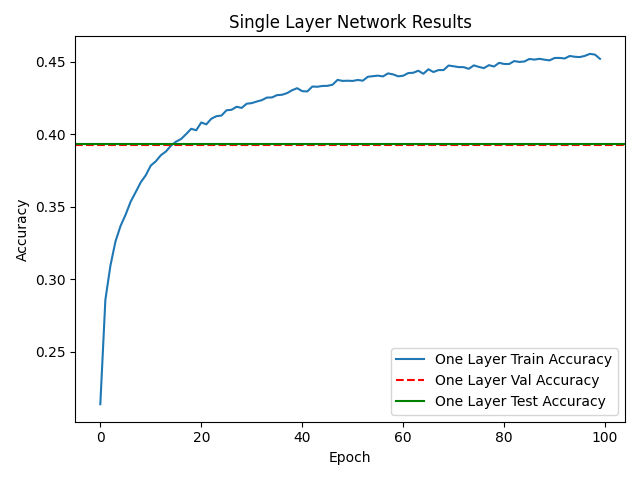
\includegraphics[width=75mm]{OneLayerResults}}
\caption{Results of training the one-layer network. Validation accuracy and Testing accuracy were checked at the end of training.}
\label{fig:oneLayerTrainResults}
\end{figure}

\begin{figure}[htbp]
\centerline{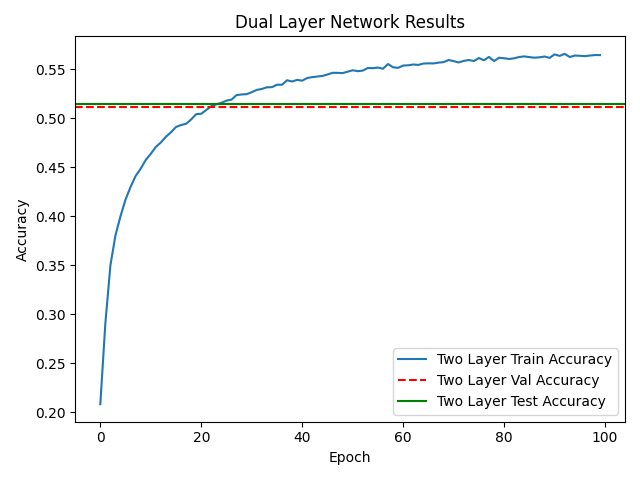
\includegraphics[width=75mm]{DualLayerResults}}
\caption{Results of training the two-layer network. Validation accuracy and Testing accuracy were checked at the end of training.}
\label{fig:dualLayerTrainResults}
\end{figure}

\begin{table}
\caption{Testing results on the A100 GPU}
\label{tab:resultsTable}
\resizebox{\columnwidth}{!}{%
    \begin{tabular}{l m{2cm} m{2cm} m{2cm} m{2cm}}
        Topology & Test Accuracy & Time Per Epoch to Train (s) & Epochs Required & Train Time (s)\\
        \hline
        Single Layer & 0.37 & 0.2464 & 20 & 4.93 \\
         Dual Layer & 0.50 & 0.307 & 40 & 12.31 \\
    \end{tabular}%
    }
\end{table}

\begin{table}
\caption{Our results compared with Keller Jordan's program}
\label{tab:jordanKellerResults}
\resizebox{\columnwidth}{!}{%
    \begin{tabular}{l m{2cm} m{2cm} }
        Attributes & Dual Layer & Jordan's Network \\
        \hline
        Accuracy & 0.50 & 0.94 \\
        Time per Epoch (s) & 0.307 & 0.383 \\
        Num Epochs & 400 & 12 \\
        Total Time to Train (s) & 12.31 & 4.6 \\
    \end{tabular}%
    }
\end{table}

\section{Discussion and Conclusion}

As is made evident by our results, we have made a functioning neural network capable of identifying images with some certainty. While this low degree of certainty compared to contemporary programs isn't very close to the ideal, it is a start for future work. Ultimately, the contemporaries make usage of many various additions and modifications to improve the quality of their image identifiers such as a convolutional layer, scale bias, image flipping, and look ahead. Of major interest to our group is look ahead, which is defined in terms of neural networks as a type of stochastic optimizer that iteratively updates two sets of weights: "fast" and "slow". Intuitively, the algorithm chooses a search direction by looking ahead at the sequence of fast weights generated by another optimizer\cite{b4}. If we were to have more time to develop this neural network, we would take a very close look at these techniques and see how they might be applied to our program and possibly passed through a kernel for parallel processing and greater upgrades in terms of the time-to-execute for our program. In addition, we wish to implement a number of additional upgrades, such as importing the dataset asynchronously, change the precision models in order to fit more information into each kernel, and possibly extending our image classifier to be used on more types of information besides just the CIFAR-10 dataset.


\section*{Acknowledgment}

Thank you to Professor Michael Gowanlock for the course knowledge and opportunity to research how the GPU can be used to implement a neural network. Additional thanks to our classmates sharing information and resources in order to overcome our team's challenges.

\begin{thebibliography}{00}
\bibitem{b1} W. W. Hwu, D. Kirk, and I. E. Hajj, Programming Massively Parallel Processors: A Hands-on Approach, 4th ed. Cambridge, MA: Morgan Kaufmann, 2023. 
\bibitem{b2} A. Krizhevsky, “The CIFAR-10 dataset,” CIFAR-10 and CIFAR-100 datasets, https://www.cs.toronto.edu/~kriz/cifar.html (accessed May 6, 2024). 
\bibitem{b3} F.-F. Li, J. Johnson, and S. Yeung, “Lecture 2 image classification,” YouTube, https://www.youtube.com/watch?v=OoUX-nOEjG0\&list=PLC1qU-LWwrF64f4QKQT-Vg5Wr4qEE1Zxk\&index=4 (accessed May 6, 2024). 
\bibitem{b4} “Papers with code - lookahead explained,” Explained Papers With Code, https://paperswithcode.com/method/lookahead\#:~:text=Lookahead\%20is \%20a\%20type\%20of,weights\%20generated\%20by\%20another \%20optimizer. (accessed May 6, 2024). 
\bibitem{b5}K. Jordan, “94\% on CIFAR-10 in 3.29 Seconds on a Single GPU,” 94\% on CIFAR-10 in 3.29 seconds on a single GPU, https://arxiv.org/html/2404.00498v1\#:~:text=To\%20accelerate\%20research \%20and\%20reduce,a\%20single\%20NVIDIA\%20A100\%20GPU (accessed May 7, 2024). 
\bibitem{b6} Alex Krizhevsky, Ilya Sutskever, and Geoffrey E. Hinton. 2012. ImageNet classification with deep convolutional neural networks. In Proceedings of the 25th International Conference on Neural Information Processing Systems - Volume 1 (NIPS'12). Curran Associates Inc., Red Hook, NY, USA, 1097–1105.

\end{thebibliography}

\appendix
\section{How to run the neural network}
To run the neural network:
\begin{enumerate}
    \item Copy the entire source code repo to Monsoon
    \item Download the binary version of the CIFAR-10 Dataset \href{https://www.cs.toronto.edu/~kriz/cifar-10-binary.tar.gz}{CIFAR-10 Dataset Download}
    \item Unzip the archive and copy the .bin files to \newline\url{~/datasets/cifar-10-batches-bin} on Monsoon. \url{~/datasets} is a directory you must create if it does not already exist. 
    \item Navigate to the \textit{src} folder and run the script by executing the command \textit{./dnn.sh}. Do not try and run the \textit{dnn.sh} shell script using the \textit{sbatch} command, it will not work. You may have to make it executable by running \newline\textit{chmod +x dnn.sh}. This script makes the executable and runs sbatch, passing in a dynamically generated sbatch file. Your username will be substituted in automatically. The script waits for the job to finish and then directly prints the output. 
\end{enumerate}

\end{document}
